\documentclass[tikz, border=10pt]{standalone}

\usetikzlibrary{arrows}
\usepackage[T1]{fontenc}
\usepackage[utf8]{inputenc}
\usepackage{lmodern}  

\begin{document}
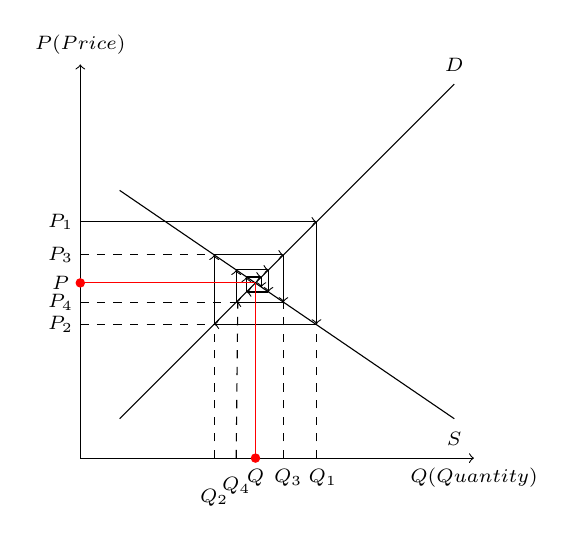
\begin{tikzpicture}
	\draw[->] (0, 0) -- (5, 0);
	\draw[->] (0, 0) -- (0, 5);

	\draw (0.5, 3.4) -- (4.75, 0.5);
	\draw (0.5, 0.5) -- (4.75, 4.75);
	
	\draw[->] (0, 3)  -- (3, 3);
	\draw[->] (3, 3) -- (3, 1.7);
	\draw[->] (3, 1.7) -- (1.7, 1.7);
	\draw[->] (1.7, 1.7) -- (1.7, 2.58);
	\draw[->] (1.7, 2.58) -- (2.58, 2.58);
	\draw[->] (2.58, 2.58) -- (2.58, 1.98);
	\draw[->] (2.58, 1.98) -- (1.98, 1.98);
	\draw[->] (1.98, 1.98) -- (1.98, 2.39);
	\draw[->] (1.98, 2.39) -- (2.39, 2.39);
	\draw[->] (2.39, 2.39) -- (2.39, 2.11);
	\draw[->] (2.39, 2.11) -- (2.11, 2.11);
	\draw[->] (2.11, 2.11) -- (2.11, 2.3);
	\draw[->] (2.11, 2.3) -- (2.3, 2.3);
	\draw[->] (2.3, 2.3) -- (2.3, 2.17);
	
	\draw[color=red] (0, 2.225) -- (2.225, 2.225);
	\draw[color=red] (2.225, 0) -- (2.225, 2.225);
	
	\draw[dashed] (0, 1.7)  -- (3, 1.7);
	\draw[dashed] (0, 1.98) -- (2, 1.98);
	\draw[dashed] (0, 2.58) -- (2, 2.58);
	
	\draw[dashed] (1.7, 0)  -- (1.7, 1.7);
	\draw[dashed] (1.98, 0) -- (2, 1.98);
	\draw[dashed] (2.58, 0) -- (2.58, 2.58);
	\draw[dashed] (3, 0) -- (3, 3);
	
		\begin{scriptsize}
			\draw [fill=red, color=red] (0, 2.225) circle (1.5pt); % P
			\draw [fill=red, color=red] (2.225, 0) circle (1.5pt); % Q
		
			\draw (0, 5.25) node {$P (Price)$};
			\draw (5, -0.25) node {$Q (Quantity)$};
			
			\draw (-0.25, 2.225) node {$P$};
			\draw (2.225, -0.25) node {$Q$};
			
			\draw (4.75, 0.25) node {$S$};
			\draw (4.75, 5) node {$D$};
			
			\draw (-0.25, 3) node {$P_{1}$};
			\draw (-0.25, 1.7) node {$P_{2}$};
			\draw (-0.25, 2.58) node {$P_{3}$};
			\draw (-0.25, 1.98) node {$P_{4}$};
			
			\draw (3.08, -0.25) node {$Q_{1}$};
			\draw (1.7, -0.5) node {$Q_{2}$};
			\draw (2.64, -0.25) node {$Q_{3}$};
			\draw (1.98, -0.35) node {$Q_{4}$};
		\end{scriptsize}
\end{tikzpicture}
\end{document}